\documentclass[tikz]{standalone}

\usetikzlibrary{patterns}

\tikzset{cross/.style={cross out, draw=black, minimum size=2*(#1-\pgflinewidth), inner sep=0pt, outer sep=0pt},
%default radius will be 1pt.
cross/.default={4pt}}


\begin{document}
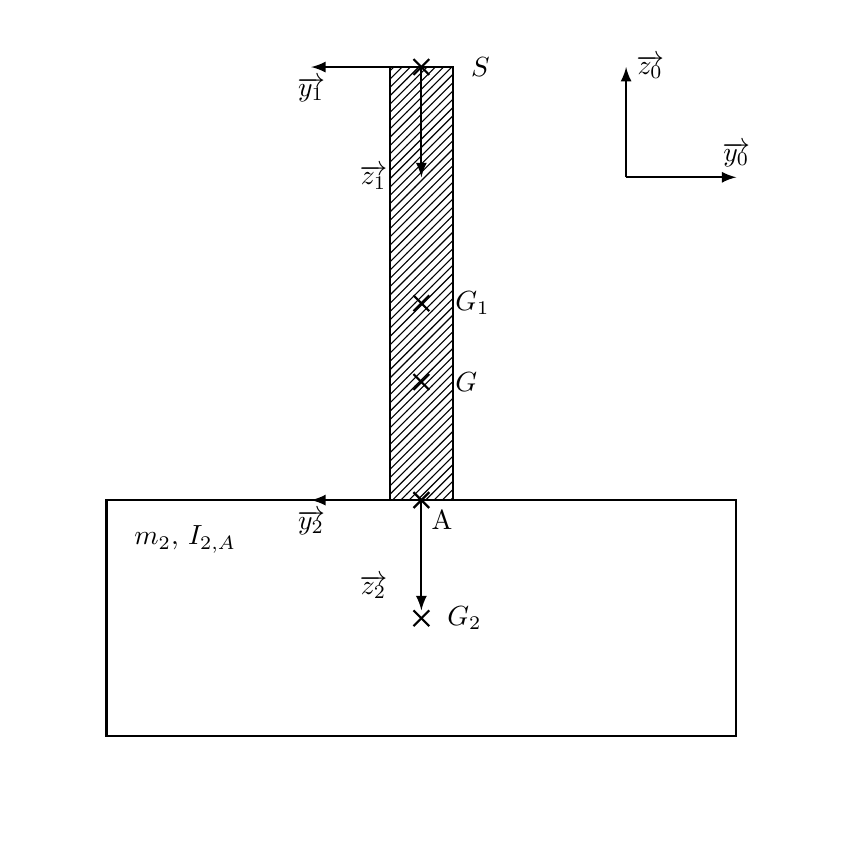
\begin{tikzpicture}[thick,>=latex,->]


\begin{scope}
\clip(-5,6) rectangle (5,-4);
% \draw[step=1cm,gray,very thin] (-5,6) grid (10,-5);

% \filldraw[white] (-4.3,4.3) rectangle (4.3,0);
% \draw[double distance=1.6mm] (0,0) -- (3,-3) node[midway,xshift=4mm,yshift=2mm]{$\ell$};
% \draw[->] (3,-3) -- (3,-4.5) node[below]{$m\cdot g$};
% \draw[->] (3,-3) -- (2.,-2.0) node[left,yshift=-3mm]{$F$};
% \draw[fill=white] (-.5,.25) -- (.5,.35) -- (1.2,0.2) -- (-1.2,-0.2) -- cycle;
% \draw[fill=white] (-.4,1) -- (-.7,.9) -- (-.3,.8) -- (-.7,.7) -- (-.3,.5) -- (-.7,.4) -- (-.5,.25) -- (.5,.35) --  (.7,.5) -- (.3,.6) -- (.7,.7) -- (.3,.8) -- (.7,.9) -- (.4,1) -- cycle;
\draw[fill=white] (-4, -3) -- (-4, 0) -- (4, 0) -- (4,-3) -- cycle;


% \draw[draw=black,fill=white] (0, 0) circle circle (.3cm);
% \draw[draw=black,fill=white] (3,-3) circle circle (.3cm);
\draw[->] (2.6,4.1) -- (4,4.1) node[above]{$\overrightarrow{y_0}$};
\draw[->] (2.6,4.1) -- (2.6,5.5) node[right]{$\overrightarrow{z_0}$};

\draw[->] (0.0,5.5) -- (-1.4,5.5) node[below]{$\overrightarrow{y_1}$};
\draw[->] (0.0,5.5) -- (0.0,4.1);
\node[left] at (-0.3,4.1) {$\overrightarrow{z_1}$};

\draw[->] (0.0,0.0) -- (-1.4,0.0) node[below]{$\overrightarrow{y_2}$};
\draw[->] (0.0,0.0) -- (0.0,-1.4);
\node[left] at (-0.3,-1.1) {$\overrightarrow{z_2}$};

% \draw[dash dot] (0,0) -- (2.55,0) node[below]{$\overrightarrow{y_0}$};
% \draw[dash dot] (0,0) -- (2.5, .42) node[above]{$\overrightarrow{y_2}$};
% \draw[thick] ([shift=(0:2cm)]0,0) arc (0:20:1cm);
% \node[] at (2.3, .2) {$\theta$};

\draw[pattern=north east lines] (-.4,5.5) rectangle (.4,0);

\node[right] at (.5,5.5) {$S$};
\draw[fill=white] (-.1, 5.4) -- (.1, 5.6) -- cycle;
\draw[fill=white] (-.1, 5.6) -- (.1, 5.4) -- cycle;

\node[below right] at (0,0) {A};
\draw[fill=white] (-.1, -.1) -- (.1, .1) -- cycle;
\draw[fill=white] (-.1, .1) -- (.1, -.1) -- cycle;

\node[right] at (0.3,1.5) {$G$};
\draw[fill=white] (-.1, 1.4) -- (.1, 1.6) -- cycle;
\draw[fill=white] (-.1, 1.6) -- (.1, 1.4) -- cycle;

\node[right] at (.2,-1.5) {$G_2$};
\draw[fill=white] (-.1, -1.6) -- (.1, -1.4) -- cycle;
\draw[fill=white] (-.1, -1.4) -- (.1, -1.6) -- cycle;

\node[right] at (0.3,2.5) {$G_1$};
\draw[fill=white] (-.1, 2.4) -- (.1, 2.6) -- cycle;
\draw[fill=white] (-.1, 2.6) -- (.1, 2.4) -- cycle;

\node[rotate=0] at (-3,-0.5) {$m_2$, $I_{2,A}$};

\end{scope}

\end{tikzpicture}
\end{document}
